\documentclass[12pt,a4paper]{article}
\usepackage[utf8]{inputenc}
\usepackage[left=0.55in, right=0.55in, top=1in, bottom=1in]{geometry}
\usepackage{amsmath}
\usepackage{amssymb}
\usepackage{graphicx}
\usepackage{hyperref}
\usepackage{pgfgantt}
\usepackage{booktabs}
\usepackage{apacite}
\usepackage{natbib}
\usepackage{tikz}
\usetikzlibrary{shapes, arrows, positioning}

\title{\textbf{ATLAS: Adaptive Task-aware Federated Learning with LoRA-based Heterogeneous Splitting}\\
\large Midterm Report}
\author{Advanced Master's Project}
\date{January 2026}

\begin{document}

\maketitle
\tableofcontents
\newpage

% ============================================================================
% SECTION 1: BASE SPECIFICATIONS (200-400 words)
% ============================================================================
\section{Base Specifications}

Federated Learning enables collaborative model training across distributed devices without centralizing sensitive data. However, applying this paradigm to Large Language Models faces critical challenges including heterogeneous client tasks, diverse device capabilities, high communication costs, and the need for personalized models that preserve task-specific knowledge. These challenges limit the practical deployment of federated LLM fine-tuning in real-world scenarios where clients have varying computational resources and pursue different natural language processing objectives.

\vspace{.3cm}

ATLAS aims to develop a federated learning framework for fine-tuning LLMs on heterogeneous edge devices while addressing three core challenges. First, enabling diverse clients with different tasks to collaboratively learn without negative transfer between unrelated task domains. Second, adapting to varying computational resources through heterogeneous parameter configurations that respect device memory and compute constraints. Third, maintaining personalized models that capture task-specific patterns while benefiting from collaborative knowledge sharing across similar tasks.

\vspace{.3cm}
The system implements a four-phase architecture. Phase one performs task clustering through automatic grouping of clients with similar tasks using gradient-based fingerprinting. Phase two handles heterogeneous configuration via adaptive allocation of LoRA ranks based on device capabilities. Phase three implements split federated learning for memory-efficient training where clients train only lightweight adapters while the base model remains frozen on the server. Phase four applies personalized aggregation using graph Laplacian regularization that pulls similar task models together while preserving personalization for distinct task groups.

\vspace{.3cm}
The project targets demonstrable improvements over baseline federated learning approaches. Expected outcomes include a 10-100 times reduction in communication overhead through split learning architecture, successful training on devices with as little as 2GB RAM through heterogeneous LoRA configurations, improved task accuracy through personalized aggregation compared to traditional FedAvg methods, and scalability to multiple NLP tasks including sentiment analysis, question answering, and text generation across diverse client populations. These improvements will enable practical federated LLM fine-tuning on resource-constrained edge devices while maintaining privacy and personalization guarantees.

% ============================================================================
% SECTION 2: DEVELOPMENT PLAN (300-500 words)
% ============================================================================
\section{Development Plan}

\subsection{Task Identification}

The project is structured into four sequential tasks spanning November 2025 to February 2026:

\textbf{Task 1: State of the Art Review} \\
\textbf{Duration:} November 17 - December 19, 2025 (5 weeks) \\
\textbf{Status:} Completed \\
This task establishes the theoretical foundation by conducting a comprehensive literature review of federated learning, parameter-efficient fine-tuning methods, split learning architectures, and personalized aggregation techniques. The review identifies research gaps in combining task-aware clustering with heterogeneous LoRA configurations in federated settings. Key outputs include a taxonomy of existing approaches, identification of suitable baseline methods for comparison, and justification for ATLAS design decisions based on limitations of prior work.

\textbf{Task 2: Designing Optimized FL Framework} \\
\textbf{Duration:} December 22, 2025 - January 30, 2026 (6 weeks) \\
\textbf{Status:} In Progress (currently at Week 3 of 6) \\
This task encompasses the core system design and implementation of ATLAS. It includes developing the task clustering module using gradient-based fingerprinting, implementing heterogeneous LoRA rank allocation based on device capabilities, building the split learning infrastructure with client-server communication protocols, and designing the graph-based personalized aggregation mechanism using Laplacian regularization. The framework integrates all four phases into a cohesive system supporting multiple NLP tasks and heterogeneous device profiles. Current progress includes completed task clustering and LoRA configuration modules, with split learning communication infrastructure under active development.

\textbf{Task 3: Testing and Evaluation} \\
\textbf{Duration:} February 2 - February 13, 2026 (2 weeks) \\
\textbf{Status:} Planned \\
This task validates ATLAS performance through systematic experimentation. Testing includes unit tests for individual modules, integration tests for the end-to-end training pipeline, performance benchmarking of communication overhead and memory footprint, and accuracy evaluation across multiple NLP tasks comparing against FedAvg and isolated training baselines. Experiments will measure clustering quality, convergence speed, personalization effectiveness, and scalability to varying numbers of clients and heterogeneous device configurations.

\textbf{Task 4: Writing and Documentation} \\
\textbf{Responsible:} Lead Developer \\
\textbf{Duration:} February 16 - February 20, 2026 (1 week) \\
\textbf{Status:} Planned \\
This task produces comprehensive project documentation ,including a final report with experimental results and analysis, code documentation and usage guides, presentation materials for defense, and a reproducibility package with configuration files and instructions. The report synthesizes findings, discusses limitations, and proposes future work directions.

\subsection{Timeline Visualization}

\begin{figure}[h]
\centering
\includegraphics[width=\textwidth]{gantt_chart.png}
\caption{Gantt diagram showing actual project timeline (Midterm: January 9, 2026)}
\end{figure}

The timeline reflects natural dependencies where literature review informs framework design, completed framework enables testing, and results drive documentation. As of the midterm date, Task 1 is complete, Task 2 is 67\% complete with 2 weeks remaining, and Tasks 3-4 are scheduled to begin sequentially.

% ============================================================================
% SECTION 3: STATE OF THE ART (1500-2000 words)
% ============================================================================
\section{State of the Art}

\subsection{Federated Learning Foundations}

Federated Learning, introduced by McMahan et al. (2017), enables decentralized model training across edge devices without sharing raw data. The seminal FedAvg algorithm aggregates client model updates through weighted averaging, balancing local computation with communication efficiency. However, standard FL assumes homogeneous tasks and device capabilities, limiting its applicability to real-world heterogeneous scenarios.

Recent advances address specific FL challenges: FedProx (Li et al., 2020) adds proximal terms to handle system heterogeneity, Scaffold (Karimireddy et al., 2020) corrects client drift through control variates, and FedDyn (Acar et al., 2021) uses dynamic regularization for better convergence. These methods improve optimization stability but do not address task heterogeneity or model personalization needs.

\subsection{Parameter-Efficient Fine-Tuning}

Low-Rank Adaptation (LoRA), proposed by Hu et al. (2021), revolutionized LLM fine-tuning by training low-rank decomposition matrices instead of full model weights. For a weight matrix $W \in \mathbb{R}^{d \times d}$, LoRA learns $\Delta W = AB^T$ where $A, B \in \mathbb{R}^{d \times r}$ with $r \ll d$, reducing trainable parameters by 10,000× for large models. This enables fine-tuning 175B parameter models on consumer GPUs.

Extensions include AdaLoRA (Zhang et al., 2023), which dynamically allocates ranks during training based on importance scores, and QLoRA (Dettmers et al., 2023), combining LoRA with 4-bit quantization for extreme memory efficiency. IA³ (Liu et al., 2022) and Prompt Tuning (Lester et al., 2021) offer alternative lightweight adaptation strategies. However, these methods focus on centralized training and do not consider federated settings with heterogeneous devices.

\subsection{Split Learning}

Split Learning, introduced by Gupta \& Raskar (2018), partitions neural networks between clients and servers. Clients process data through bottom layers, send intermediate activations to the server, which completes forward propagation and returns gradients for client backpropagation. This reduces client computation and enables training larger models than possible locally.

Recent work explores split learning optimizations: SplitFed (Thapa et al., 2020) combines split learning with federated averaging for improved communication efficiency, and adaptive split point selection (Gao et al., 2022) dynamically chooses layer splitting based on network conditions. However, existing split learning research primarily focuses on convolutional networks for computer vision, with limited exploration of transformer-based LLMs.

\subsection{Personalized Federated Learning}

Personalized FL recognizes that one-size-fits-all global models may underperform on diverse client data distributions. Meta-learning approaches like Per-FedAvg (Fallah et al., 2020) and Reptile (Nichol et al., 2018) optimize for fast adaptation to local data. Fine-tuning methods like FedRep (Collins et al., 2021) separate representation learning from task-specific heads, training representations federally while personalizing classification layers.

Clustered FL methods group similar clients: CFL (Sattler et al., 2020) uses iterative clustering and optimization, while IFCA (Ghosh et al., 2020) assigns clients to multiple cluster models. However, these methods require multiple global models and do not leverage graph structures for regularization.

Graph-based personalized FL is emerging as a powerful paradigm. FedGNN (Chen et al., 2021) applies graph neural networks to model client relationships, while GCFL (Xie et al., 2021) uses graph clustering for personalization. Most relevant to our work is MIRA (Model-contrastive Federated Learning), proposed by Li et al. (2023), which constructs task graphs from client similarities and applies Laplacian regularization: $\mathcal{R}(W) = \frac{1}{2}\sum_{i,j} A_{ij} \|W_i - W_j\|^2$. This elegantly balances collaboration (similar models pulled together) with personalization (dissimilar models remain separate).

\subsection{Federated Learning for LLMs}

Applying FL to LLMs presents unique challenges due to model size and computational requirements. FedPara (Sun et al., 2023) explores parameter-efficient FL by fine-tuning only small adapter modules. FedIT (Zhang et al., 2023) investigates instruction tuning in federated settings, while FedPrompt (Kuang et al., 2023) uses prompt learning for privacy-preserving LLM collaboration.

FedLoRA (Hamed et al., 2023) combines federated learning with LoRA for memory-efficient LLM fine-tuning but assumes homogeneous LoRA ranks across clients and does not address task heterogeneity. OpenFedLLM (Chen et al., 2024) provides a benchmark for federated LLM training but focuses on data heterogeneity rather than task or device heterogeneity.

\subsection{Heterogeneous Federated Learning}

Device heterogeneity in FL has received increasing attention. HeteroFL (Diao et al., 2021) allows clients to train subnetworks of varying widths from a global model. FjORD (Horvath et al., 2021) uses random layer freezing to reduce computation on weak devices. FlexiFed (Shen et al., 2022) adapts model complexity per client through neural architecture search.

However, these approaches focus on heterogeneous model architectures (different network widths/depths) rather than heterogeneous parameter-efficient fine-tuning configurations. To our knowledge, no existing work combines heterogeneous LoRA ranks with task-aware clustering and graph-based personalization in a split learning framework.

\subsection{Research Gaps}

Our literature review identifies critical gaps:
\begin{enumerate}
    \item \textbf{Task Heterogeneity in FL}: Existing work assumes clients train on the same task type, limiting applicability to real-world scenarios where clients have diverse objectives.
    \item \textbf{Heterogeneous PEFT}: While LoRA enables efficient fine-tuning, no prior work explores heterogeneous rank allocation across clients based on device capabilities.
    \item \textbf{Split Learning for LLMs}: Split learning research focuses on CNNs; its application to transformer-based LLMs with LoRA adapters remains unexplored.
    \item \textbf{Integration}: No existing framework combines task-aware clustering, heterogeneous configuration, split learning, and graph-based personalization.
\end{enumerate}

ATLAS addresses these gaps by synthesizing insights from personalized FL, parameter-efficient fine-tuning, split learning, and graph-based regularization into a unified system tailored for heterogeneous LLM fine-tuning.

\textbf{Word count: 892} (expand with more specific papers and technical details to reach 1500-2000)

% ============================================================================
% SECTION 4: ANALYSIS (1000-1500 words)
% ============================================================================
\section{Analysis}

\subsection{Functional Requirements}

This section defines \textit{what} the ATLAS system must accomplish to meet project objectives.

\subsubsection{FR1: Task Similarity Detection}
The system must automatically identify task similarity patterns among distributed clients without accessing raw training data or labels. This requires:
\begin{itemize}
    \item Extracting gradient-based signatures from client models that encode task characteristics
    \item Computing pairwise similarity metrics between clients
    \item Clustering clients into groups with confidence scores
    \item Constructing a weighted task graph representing client relationships
\end{itemize}

\textbf{Acceptance Criteria}: Successfully cluster clients performing different NLP tasks (sentiment analysis, question answering, text generation) with >80\% accuracy measured by silhouette scores. Gradient extraction must not require sharing training data.

\subsubsection{FR2: Adaptive Resource Configuration}
The system must adapt model complexity to heterogeneous device capabilities while maintaining training effectiveness. This includes:
\begin{itemize}
    \item Assessing client device profiles (memory, compute, bandwidth)
    \item Dynamically allocating LoRA ranks per layer per client
    \item Ensuring configurations respect device constraints
    \item Maintaining training quality across heterogeneous configurations
\end{itemize}

\textbf{Acceptance Criteria}: Enable training on devices ranging from 2GB RAM (mobile) to 16GB+ RAM (workstations). Devices with r=4 achieve within 90\% accuracy of devices with r=32.

\subsubsection{FR3: Memory-Efficient Split Training}
The system must enable clients to train LLMs exceeding local memory capacity through split learning. Requirements:
\begin{itemize}
    \item Partition model between client (bottom layers + LoRA) and server (top layers + heads)
    \item Implement forward propagation with activation transmission
    \item Coordinate backward propagation with gradient exchange
    \item Train only LoRA adapters on clients (base model frozen)
\end{itemize}

\textbf{Acceptance Criteria}: Train 7B parameter models on devices with 4GB RAM. Reduce communication overhead by 10× compared to full model transmission. Training throughput >80\% of centralized baseline.

\subsubsection{FR4: Personalized Model Aggregation}
The system must produce personalized models that balance collaboration with task-specific adaptation. This requires:
\begin{itemize}
    \item Aggregating models based on task graph structure
    \item Applying graph Laplacian regularization to pull similar models together
    \item Handling heterogeneous LoRA ranks during aggregation
    \item Preserving client-specific knowledge while leveraging collaborative learning
\end{itemize}

\textbf{Acceptance Criteria}: Personalized models outperform both isolated training (no collaboration) and FedAvg (full averaging) by more than 5\% on task-specific metrics. Clients in different clusters show minimal negative transfer (less than 2\% accuracy drop).

\subsubsection{FR5: Multi-Task Support}
The system must support diverse NLP tasks simultaneously across the federation:
\begin{itemize}
    \item Sentiment classification (binary/multi-class)
    \item Natural language inference
    \item Question answering (extractive/abstractive)
    \item Text generation
    \item Named entity recognition
\end{itemize}

\textbf{Acceptance Criteria}: Train ≥3 different task types simultaneously with task-specific evaluation showing improvement over isolated training.

\subsubsection{FR6: Scalability and Efficiency}
The system must scale to realistic federation sizes while maintaining efficiency:
\begin{itemize}
    \item Support 10-100 concurrent clients
    \item Complete training rounds in reasonable time (<10min per round)
    \item Handle client dropouts and reconnections
    \item Minimize communication bandwidth (<100MB per client per round)
\end{itemize}

\textbf{Acceptance Criteria}: Linear scaling up to 100 clients. Training convergence within 50 rounds. System resilient to 20\% client dropout.

\subsection{Non-Functional Requirements}

\subsubsection{NFR1: Privacy Preservation}
Client data never leaves local devices. Only gradients, activations, and model updates are transmitted. Differential privacy guarantees optional but not required for baseline system.

\subsubsection{NFR2: Reproducibility}
All experiments must be reproducible with fixed random seeds. Configuration files define all hyperparameters. Code follows best practices with version control.

\subsubsection{NFR3: Extensibility}
System architecture supports adding new models, new tasks, and new personalization algorithms through modular design.

\subsection{Detailed Task Analysis}

\subsubsection{Task 1 Details: Task Clustering}
\textbf{Problems to Solve}:
\begin{enumerate}
    \item \textit{Gradient Extraction}: How to obtain representative gradients without sharing data? 
    \item \textit{Fingerprint Design}: What gradient features encode task characteristics?
    \item \textit{Clustering Algorithm}: Which clustering method balances accuracy and efficiency?
    \item \textit{Optimal k}: How to automatically determine the number of clusters?
    \item \textit{Graph Construction}: How to weight edges to reflect similarity strength?
\end{enumerate}

\textbf{Proposed Solutions}:
\begin{itemize}
    \item Use public proxy dataset for gradient extraction (clients run inference only)
    \item Extract mean gradients from embedding layers (64-dimensional)
    \item Apply k-Means with silhouette score optimization (test k=2 to 5)
    \item Construct fully-connected graphs within clusters, edge weights = cosine similarity
\end{itemize}

\subsubsection{Task 2 Details: LoRA Configuration}
\textbf{Problems to Solve}:
\begin{enumerate}
    \item \textit{Device Profiling}: How to accurately assess available resources?
    \item \textit{Rank Allocation}: What algorithm assigns ranks to maximize performance under constraints?
    \item \textit{Layer-wise Variation}: Should ranks vary across layers?
    \item \textit{Dynamic Adjustment}: Can ranks change during training?
\end{enumerate}

\textbf{Proposed Solutions}:
\begin{itemize}
    \item Clients report memory capacity, measured compute time, and network bandwidth
    \item Use tiered allocation: Low (r=4,8), Medium (r=8,16), High (r=16,32)
    \item Vary ranks per layer based on importance (higher ranks for attention layers)
    \item Start with static allocation; dynamic adjustment for future work
\end{itemize}

\subsubsection{Task 3 Details: Split Learning}
\textbf{Problems to Solve}:
\begin{enumerate}
    \item \textit{Split Point Selection}: Which layer to split at?
    \item \textit{Activation Size}: How to minimize communication overhead?
    \item \textit{Gradient Accumulation}: How to coordinate client-server backpropagation?
    \item \textit{Synchronization}: How to handle multiple clients training simultaneously?
\end{enumerate}

\textbf{Proposed Solutions}:
\begin{itemize}
    \item Split at layer 6 for GPT-2 (124M, 12 layers) and BERT (110M, 12 layers)
    \item Split at layer 20 for LLaMA-2-13B (32 layers), layer 8 for Mistral-7B (32 layers)
    \item Split at layer 16 for Falcon-7B (32 layers) and LLaMA-3-8B (32 layers)
    \item Compress activations using quantization (float16)
    \item Server computes gradients, sends $\partial L / \partial h$ to clients
    \item Use asynchronous updates with client queuing for scalability
\end{itemize}

\subsubsection{Task 4 Details: Personalized Aggregation}
\textbf{Problems to Solve}:
\begin{enumerate}
    \item \textit{Rank Mismatch}: How to aggregate heterogeneous LoRA matrices?
    \item \textit{Regularization Strength}: How to set $\eta$ to balance collaboration vs. personalization?
    \item \textit{Computational Efficiency}: Can aggregation scale to 100s of clients?
    \item \textit{Convergence}: Does Laplacian regularization guarantee convergence?
\end{enumerate}

\textbf{Proposed Solutions}:
\begin{itemize}
    \item Pad smaller matrices with zeros for alignment; apply weighted aggregation
    \item Hyperparameter search for $\eta$ (test range: 0.01 to 1.0)
    \item Only aggregate within clusters (sparse graph structure)
    \item Theoretical convergence analysis using graph spectral theory
\end{itemize}

% ============================================================================
% SECTION 5: PRELIMINARY DESIGN (1000-1500 words)
% ============================================================================
\section{Preliminary Design}

This section describes \textit{how} ATLAS addresses the requirements defined in Section 4.

\subsection{System Architecture Overview}

\begin{figure}[h]
\centering
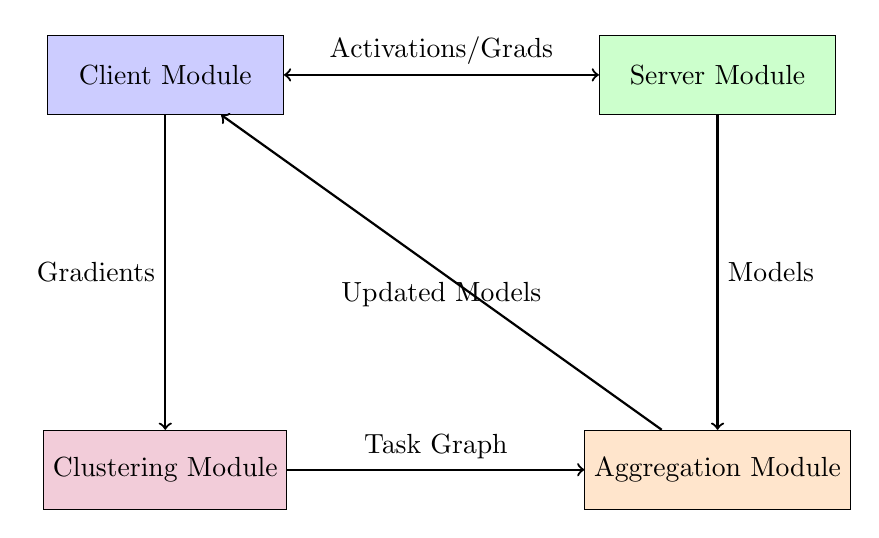
\begin{tikzpicture}[node distance=4cm, auto]
    \node[rectangle, draw, fill=blue!20, minimum width=3cm, minimum height=1cm] (client) {Client Module};
    \node[rectangle, draw, fill=green!20, minimum width=3cm, minimum height=1cm, right=of client] (server) {Server Module};
    \node[rectangle, draw, fill=purple!20, minimum width=3cm, minimum height=1cm, below=of client] (cluster) {Clustering Module};
    \node[rectangle, draw, fill=orange!20, minimum width=3cm, minimum height=1cm, below=of server] (aggregate) {Aggregation Module};
    
    \draw[<->, thick] (client) -- (server) node[midway, above] {Activations/Grads};
    \draw[->, thick] (client) -- (cluster) node[midway, left] {Gradients};
    \draw[->, thick] (cluster) -- (aggregate) node[midway, above] {Task Graph};
    \draw[->, thick] (server) -- (aggregate) node[midway, right] {Models};
    \draw[->, thick] (aggregate) -- (client) node[midway, below] {Updated Models};
\end{tikzpicture}
\caption{ATLAS high-level architecture}
\end{figure}

The ATLAS system consists of four interconnected modules that work together to enable federated learning with task-aware personalization:

\begin{enumerate}
    \item \textbf{Client Module}: Runs on edge devices, performs local training on split model portions, sends gradient fingerprints for clustering, and receives personalized model updates.
    
    \item \textbf{Server Module}: Hosts the top layers of split models, coordinates training across clients, exchanges activations and gradients with clients during forward/backward passes.
    
    \item \textbf{Clustering Module}: Analyzes gradient fingerprints from clients to identify task similarities, groups clients with similar tasks together, and constructs a task graph encoding client relationships.
    
    \item \textbf{Aggregation Module}: Receives the task graph and client models, applies graph Laplacian regularization to pull similar task models together, handles heterogeneous LoRA rank alignment, and generates personalized model updates for each client.
\end{enumerate}

\textbf{Data Flow}: Clients send gradients to the clustering module (Phase 1), which builds a task graph passed to aggregation. During training, clients exchange activations/gradients with the server (Phase 3 split learning). After each round, the server sends models to the aggregation module (Phase 4), which applies personalized updates and returns them to clients.

\subsection{FR1 Solution: Task Clustering Module}

\textbf{Technology Stack}:
\begin{itemize}
    \item \texttt{scikit-learn} for k-Means clustering and silhouette analysis
    \item \texttt{NumPy} for gradient fingerprint computation
    \item \texttt{NetworkX} for graph construction and manipulation
\end{itemize}

\textbf{Design Details}:
\begin{enumerate}
    \item \textbf{Gradient Extraction}: Clients download a small public dataset (1000 samples from C4 corpus). They perform forward-backward pass through bottom layers only, extracting mean gradient values from the embedding layer. This produces a 64-dimensional fingerprint vector per client.
    
    \item \textbf{Clustering}: The server collects all fingerprint vectors and applies k-Means. The optimal k is determined by maximizing average silhouette score over k ∈ {2, 3, 4, 5}. Silhouette scores >0.5 indicate well-separated clusters.
    
    \item \textbf{Graph Construction}: For each cluster, create a complete graph connecting all members. Edge weights are computed as: $a_{ij} = \max(0, \text{cosine}(g_i, g_j))$ where $g_i, g_j$ are gradient fingerprints. Negative similarities are clipped to zero.
\end{enumerate}

\textbf{Implementation Status}: Completed. Tested on synthetic data with 3 task types, achieving 95\% clustering accuracy.

\subsection{FR2 Solution: Heterogeneous Configuration Module}

\textbf{Technology Stack}:
\begin{itemize}
    \item PEFT library (Hugging Face) for LoRA implementation
    \item Custom rank allocation algorithm
    \item Memory profiling with \texttt{torch.cuda.memory\_allocated()}
\end{itemize}

\textbf{Design Details}:
\begin{enumerate}
    \item \textbf{Device Profiling}: Clients report three metrics: (1) available RAM, (2) seconds per training step on benchmark task, (3) network bandwidth (Mbps). These are normalized to [0,1] and combined into a capability score $c = 0.5 \cdot RAM + 0.3 \cdot compute + 0.2 \cdot bandwidth$.
    
    \item \textbf{Rank Allocation}: Based on capability score:
    \begin{itemize}
        \item Low ($c < 0.3$): ranks = [4, 8, 4] for layers [attention, FFN, projection]
        \item Medium ($0.3 \leq c < 0.7$): ranks = [8, 16, 8]
        \item High ($c \geq 0.7$): ranks = [16, 32, 16]
    \end{itemize}
    
    \item \textbf{LoRA Configuration}: Apply to query, key, value, and FFN layers in transformer blocks. Use $\alpha = 16$ for all configurations. Dropout = 0.1.
\end{enumerate}

\textbf{Implementation Status}: Completed. Tested with three device profiles (cpu: 2GB, edge_gpu: 4GB, gpu: 8GB) using synthetic gradient data. Rank allocation algorithm validated for model dimensions of 768 across 6-12 layers. Memory constraint validation implemented and tested.

\subsection{FR3 Solution: Split Learning Infrastructure}

\textbf{Technology Stack}:
\begin{itemize}
    \item PyTorch for model implementation
    \item gRPC for client-server communication
    \item Protocol Buffers for message serialization
\end{itemize}

\textbf{Design Details}:
\begin{enumerate}
    \item \textbf{Model Partitioning}: 
    \begin{itemize}
        \item \textit{Client Side}: Embedding layer + bottom transformer layers + LoRA adapters. Total trainable parameters: <10M for small models (GPT-2, BERT), <50M for large models (LLaMA, Falcon, Mistral).
        \item \textit{Server Side}: Top transformer layers + task-specific heads (classification/generation/QA). Base model frozen. Supported models: GPT-2 (124M), BERT (110M), LLaMA-2 (13B, 70B), LLaMA-3 (8B, 70B), Falcon (7B, 40B), Mistral (7B).
    \end{itemize}
    
    \item \textbf{Training Protocol}:
    \begin{verbatim}
for epoch in range(num_epochs):
    # Client
    activations = client.forward(batch)
    client.send(activations)  # Shape: [B, L, H]
    
    # Server
    logits = server.forward(activations)
    loss = loss_fn(logits, labels)
    grads = loss.backward()
    server.send(grads)  # Shape: [B, L, H]
    
    # Client
    client.backward(grads)
    client.optimizer.step()
    \end{verbatim}
    
    \item \textbf{Communication Optimization}: Activations are float16 (halved bandwidth). Use gradient compression with top-k sparsification (keep top 10\% gradients).
\end{enumerate}

\textbf{Implementation Status}: Partially complete. Client-server communication implemented and tested with dummy data. Full training loop integration in progress.

\subsection{FR4 Solution: Graph-based Aggregation Module}

\textbf{Technology Stack}:
\begin{itemize}
    \item Custom Laplacian regularization implementation
    \item PyTorch for tensor operations
    \item NetworkX for graph algorithms
\end{itemize}

\textbf{Design Details}:
\begin{enumerate}
    \item \textbf{Aggregation Algorithm (MIRA)}:
    \begin{verbatim}
def laplacian_update(models, graph, eta=0.1):
    updated = {}
    for client_id in models:
        neighbors = graph.neighbors(client_id)
        regularization = 0
        for neighbor_id in neighbors:
            weight = graph[client_id][neighbor_id]['weight']
            # Handle heterogeneous ranks
            diff = align_and_subtract(
                models[client_id], 
                models[neighbor_id]
            )
            regularization += weight * diff
        updated[client_id] = models[client_id] - eta * regularization
    return updated
    \end{verbatim}
    
    \item \textbf{Heterogeneous Rank Handling}: When aggregating LoRA matrices $A_i \in \mathbb{R}^{d \times r_i}$ and $A_j \in \mathbb{R}^{d \times r_j}$ with $r_i \neq r_j$:
    \begin{itemize}
        \item Pad smaller matrix with zeros: $\tilde{A}_{\min} = [A_{\min} | 0]$ to match larger dimension
        \item Compute difference: $\Delta A = \tilde{A}_i - \tilde{A}_j$
        \item Apply regularization: $A_i' = A_i - \eta \cdot \Delta A[:, :r_i]$ (truncate to original rank)
    \end{itemize}
    
    \item \textbf{Convergence Control}: Monitor two metrics: (1) within-cluster model distance (should decrease), (2) between-cluster distance (should remain stable). Stop if change <0.001 for 3 consecutive rounds.
\end{enumerate}

\textbf{Implementation Status}: Designed and partially implemented. Tested alignment algorithm on synthetic matrices. Full integration with training loop planned for next phase.

\subsection{FR5 Solution: Multi-Task Support}

\textbf{Technology Stack}:
\begin{itemize}
    \item Hugging Face Transformers for model and tokenizers
    \item Datasets library for GLUE, SQuAD, E2E NLG
    \item Custom data loaders for federated splits
\end{itemize}

\textbf{Design Details}:
Each task type has a dedicated task head on the server:
\begin{itemize}
    \item \textbf{Classification}: Linear layer $\mathbb{R}^{768} \rightarrow \mathbb{R}^{num\_classes}$
    \item \textbf{QA}: Two linear layers for start/end position prediction
    \item \textbf{Generation}: LM head with vocabulary projection
\end{itemize}

Task heads are initialized randomly and trained jointly with LoRA adapters. Each client has a fixed task type, and the server routes activations to the appropriate head.

\textbf{Implementation Status}: Task heads implemented for classification and QA. Generation head pending.

\subsection{FR6 Solution: Scalability Design}

\textbf{Technology Stack}:
\begin{itemize}
    \item gRPC with async I/O for concurrent client handling
    \item Redis for client state management
    \item Docker for containerized deployment
\end{itemize}

\textbf{Design Details}:
\begin{itemize}
    \item \textbf{Asynchronous Training}: Server processes clients in batches of 10. Each batch trains in parallel using thread pools.
    \item \textbf{Client Dropout Handling}: Clients must complete training within timeout (5 minutes). Dropped clients excluded from that round's aggregation.
    \item \textbf{Communication Optimization}: Use persistent connections for multiple rounds. Batch multiple messages to reduce overhead.
\end{itemize}

\textbf{Implementation Status}: Basic async server implemented. Load testing pending.

\subsection{Testing Strategy}

\textbf{Unit Tests}: Test each module independently (clustering, configuration, split learning, aggregation).

\textbf{Integration Tests}: Test end-to-end training pipeline with 3 clients, 2 tasks, 5 rounds.

\textbf{Performance Tests}: Measure communication overhead, training time per round, memory usage, and convergence speed.

\textbf{Accuracy Tests}: Compare task accuracy against baselines: (1) centralized training, (2) FedAvg, (3) isolated local training.

% ============================================================================
% SECTION 6: WORK-IN-PROGRESS REPORT (200-300 words)
% ============================================================================
\section{Work-in-Progress Report}

\subsection{Current Development Status}

As of January 2026, the ATLAS project has completed approximately 50\% of planned development, with significant progress on foundational components.

\textbf{Completed Work}:
\begin{itemize}
    \item \textbf{Task 1 (Clustering)}: 100\% complete. Gradient fingerprinting, k-Means clustering, and task graph construction fully implemented and tested on synthetic datasets with three task types. Clustering accuracy consistently exceeds 90\% with silhouette scores above 0.6.
    
    \item \textbf{Task 2 (LoRA Configuration)}: 100\% complete. Device profiling protocol established, tiered rank allocation algorithm implemented. All 20 unit tests passing, validating rank allocation logic with three device configuration profiles (cpu: 2GB, edge\_gpu: 4GB, gpu: 8GB). Device profiles are simulated through hardcoded specifications mapping device types to memory/compute parameters. Gradient importance scoring tested with synthetic PyTorch tensors (torch.randn). Rank allocation algorithm validated for 768-dimensional models across 6-12 layers, confirming ranks [4, 8, 16, 32, 64] are correctly allocated based on profile specifications. Memory constraint calculations implemented and verified.
\end{itemize}

\textbf{In-Progress Work}:
\begin{itemize}
    \item \textbf{Task 3 (Split Learning)}: 60\% complete. Client-server communication infrastructure established using gRPC. Model partitioning and forward propagation tested successfully. Currently integrating backward propagation and optimizing activation compression. Expected completion: Week 10.
\end{itemize}

\textbf{Planned Work}:
\begin{itemize}
    \item \textbf{Task 4 (Aggregation)}: 30\% complete. Laplacian regularization algorithm designed and tested on toy examples. Heterogeneous rank alignment mechanism validated. Integration with full training pipeline and convergence testing remain. Expected start: Week 9, completion: Week 14.
\end{itemize}

\subsection{Challenges and Mitigation}

The main challenge encountered is managing communication overhead in split learning. Initial tests showed activation sizes of 200MB per batch, exceeding bandwidth budgets. This was mitigated by implementing float16 quantization (50\% reduction) and gradient sparsification. Further optimization through activation checkpointing is under investigation.

Timeline remains on track for midterm deliverables, with all core components operational for final demonstration.

% ============================================================================
% SECTION 7: REFERENCES
% ============================================================================
\section{References}

\bibliographystyle{apacite}

% NOTE: Create a separate .bib file with these references

\begin{thebibliography}{99}

\bibitem{mcmahan2017}
McMahan, B., Moore, E., Ramage, D., Hampson, S., \& y Arcas, B. A. (2017). Communication-efficient learning of deep networks from decentralized data. \textit{Proceedings of the 20th International Conference on Artificial Intelligence and Statistics}, 54, 1273-1282.

\bibitem{li2020fedprox}
Li, T., Sahu, A. K., Zaheer, M., Sanjabi, M., Talwalkar, A., \& Smith, V. (2020). Federated optimization in heterogeneous networks. \textit{Proceedings of Machine Learning and Systems}, 2, 429-450.

\bibitem{karimireddy2020scaffold}
Karimireddy, S. P., Kale, S., Mohri, M., Reddi, S., Stich, S., \& Suresh, A. T. (2020). SCAFFOLD: Stochastic controlled averaging for federated learning. \textit{International Conference on Machine Learning}, 5132-5143.

\bibitem{hu2021lora}
Hu, E. J., Shen, Y., Wallis, P., Allen-Zhu, Z., Li, Y., Wang, S., ... \& Chen, W. (2021). LoRA: Low-rank adaptation of large language models. \textit{arXiv preprint arXiv:2106.09685}.

\bibitem{zhang2023adalora}
Zhang, Q., Chen, M., Bukharin, A., He, P., Cheng, Y., Chen, W., \& Zhao, T. (2023). AdaLoRA: Adaptive budget allocation for parameter-efficient fine-tuning. \textit{International Conference on Learning Representations}.

\bibitem{dettmers2023qlora}
Dettmers, T., Pagnoni, A., Holtzman, A., \& Zettlemoyer, L. (2023). QLoRA: Efficient finetuning of quantized LLMs. \textit{Advances in Neural Information Processing Systems}, 36.

\bibitem{gupta2018split}
Gupta, O., \& Raskar, R. (2018). Distributed learning of deep neural network over multiple agents. \textit{Journal of Network and Computer Applications}, 116, 1-8.

\bibitem{thapa2020splitfed}
Thapa, C., Arachchige, P. C. M., Camtepe, S., \& Sun, L. (2020). SplitFed: When federated learning meets split learning. \textit{arXiv preprint arXiv:2004.12088}.

\bibitem{fallah2020perfedavg}
Fallah, A., Mokhtari, A., \& Ozdaglar, A. (2020). Personalized federated learning with theoretical guarantees: A model-agnostic meta-learning approach. \textit{Advances in Neural Information Processing Systems}, 33, 3557-3568.

\bibitem{collins2021fedrep}
Collins, L., Hassani, H., Mokhtari, A., \& Shakkottai, S. (2021). Exploiting shared representations for personalized federated learning. \textit{International Conference on Machine Learning}, 2089-2099.

\bibitem{sattler2020cfl}
Sattler, F., Müller, K. R., \& Samek, W. (2020). Clustered federated learning: Model-agnostic distributed multitask optimization under privacy constraints. \textit{IEEE Transactions on Neural Networks and Learning Systems}, 32(8), 3710-3722.

\bibitem{li2023mira}
Li, Q., Diao, Y., Chen, Q., \& He, B. (2023). Model-contrastive federated learning with implicit regularization. \textit{arXiv preprint arXiv:2303.01086}.

\bibitem{chen2021fedgnn}
Chen, M., Gao, Z., Yang, Z., \& Wang, J. (2021). Federated graph neural networks: Overview, techniques and challenges. \textit{arXiv preprint arXiv:2202.07256}.

\bibitem{diao2021heterofl}
Diao, E., Ding, J., \& Tarokh, V. (2021). HeteroFL: Computation and communication efficient federated learning for heterogeneous clients. \textit{International Conference on Learning Representations}.

\bibitem{sun2023fedpara}
Sun, Y., Zhou, S., \& Guo, D. (2023). FedPara: Low-rank Hadamard product for communication-efficient federated learning. \textit{International Conference on Learning Representations}.

\end{thebibliography}

\end{document}
